\begin{figure}[H]
\centering
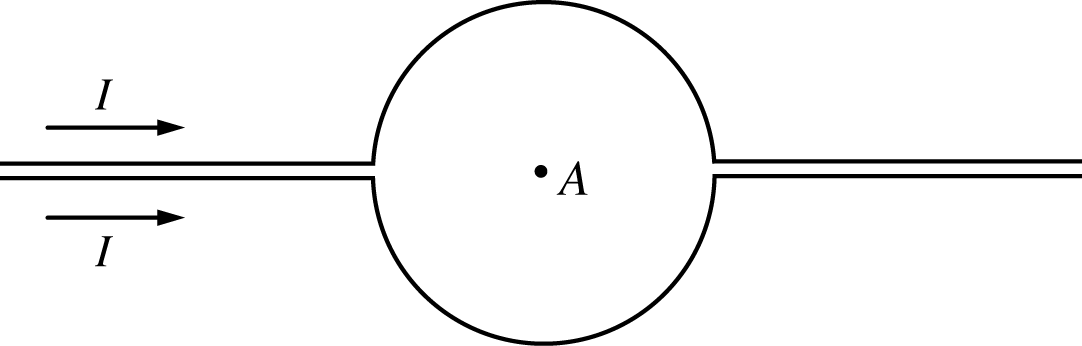
\includegraphics[scale=0.3]{images/img-008-014.png}
\end{figure}

% Multiple Choice Question 20
\begin{questions}\setcounter{question}{19}\question
The middle sections of two long, straight wires are each bent into semicircular shapes. The two wires are placed close to each other in a plane as shown above. Point $A$ is the center of the circle formed by the two wires. There is a current $I$ in each wire. Which of the following best represents the direction of the magnetic field, if any, at point A due to the currents?

\begin{choices}
\choice \adjustbox{valign=t}{
\includegraphics[scale=0.3]{images/img-008-015.png}}
\choice \adjustbox{valign=t}{
\includegraphics[scale=0.3]{images/img-008-016.png}}
\choice \adjustbox{valign=t}{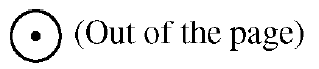
\includegraphics[scale=0.5]{images/20.3.png}}
\choice \adjustbox{valign=t}{
\includegraphics[scale=0.3]{images/img-008-018.png}}
\choice There is no direction, because the magnetic
field is zero.
\end{choices}\end{questions}
